\section{Algorithm Performance Dataset}

{\bf Attributes:} Algorithm, Epoch, Accuracy, Trial Number\\

{\bf Scenario:} You are testing two reinforcement learning (RL) algorithms on a sequential decision task. To avoid overfitting and simulate real-world noise, you shuffle the dataset for each trial and run 10 independent trials per algorithm. For each trial, you track the accuracy across 10 training epochs (one pass through a dataset). Due to how you shuffle your data and algorithmic stochasticity, accuracy results vary across trials.\\

{\bf  Research Question:} Which algorithm performs more accurately on average across epochs, and how does the use of a visualization help you assess reliability and variation of each algorithm?

\subsection{Part A: Data Cleaning and Preprocessing}
First, filter your dataset so that only the variables critical for your analysis remain. Then clean your data so that there is consistency in variable types, capitalization, and handle any missing or invalid values.\\
-----\\
The scenario specified that we are interested in epochs 1-10 over 10 trials, so we first filtered out any epochs and/or runs beyond that, for which there was one epoch 11 in the raw data. After also dropping any rows with missing accuracies, for which there were a few, we then finished by standardizing the format of the Algorithms columns and renaming the columns, to be consistent with the other two clean datasets.\\

The Algorithms column had inconcsistent casing of the word 'Algorithm', which is also irrelevant entirely to grabbing the information of which algorithm we are observing, so the casing was standardized and the term was removed from all of the values in this row. There was also whitespace in some cases, so each record was stripped, and we were left with clean 'a'/'b' labels to work with.\\

Below is the corresponding utility function:\\
 
\begin{verbatim}
def clean_preprocess_algorithms_data(input_csv: str, output_csv: str) -> pd.DataFrame:
    """
    Cleans and preprocesses the algorithms dataset by constraining the trials and epochs
    to the first 10 and then cleans the inconsistent entry of algorithm labels.

    :param input_csv:: Path to the input CSV file containing the algorithm trials dataset.
    :type input_csv: str
    :param output_csv: Filename for the clean data.
    :type output_csv: str
    :returns: pd.DataFrame
    :rtype: pd.DataFrame
    """
    df = pd.read_csv(input_csv)

    df.dropna(inplace=True)
    df = df.loc[:, ['Epoch', 'Algorithm', 'Run', 'Accuracy']]

    # Contrains to trial and epoch values within 1-10
    df = df[(df['Epoch'] >= 1) & (df['Epoch'] <= 10)]
    df = df[(df['Run'] >= 1) & (df['Run'] <= 10)]

    # Standardizes algorithms att value format
    df['Algorithm'] = df['Algorithm'].str.strip()
    df['Algorithm'] = df['Algorithm'].str.lower()
    df['Algorithm'] = df['Algorithm'].str.replace('algorithm ', '')

    df.columns = ['epoch', 'algorithm', 'run', 'accuracy']

    os.makedirs(f'../datasets/clean/', exist_ok=True)
    df.to_csv(f'../datasets/clean/{output_csv}', index=False)
    return df
\end{verbatim}

\begin{center}
\textbf{Figure 11:} Algorithm Performance data pre-processing function.
\end{center}

Below is a comparison for this dataset to illustrate the changes:\\

\noindent\textbf{algorithm\_trials.csv}
\begin{verbatim}
,Epoch,Algorithm,Run,Accuracy
0,1, algorithm a ,1,0.0464
1,2, algorithm a ,1,0.0069
2,3, algorithm a ,1,0.0992
3,4, algorithm a ,1,0.241
4,5, algorithm a ,1,
5,6, algorithm a ,1,0.4813
6,7, algorithm a ,1,0.8574
7,8, algorithm a ,1,0.9422
8,9, algorithm a ,1,0.915
9,10, algorithm a ,1,1.0
...
\end{verbatim}

\noindent\textbf{algo\_accuracy\_by\_epoch.csv}
\begin{verbatim}
epoch,algorithm,run,accuracy
1,a,1,0.0464
2,a,1,0.0069
3,a,1,0.0992
4,a,1,0.241
6,a,1,0.4813
7,a,1,0.8574
8,a,1,0.9422
9,a,1,0.915
10,a,1,1.0
1,a,2,0.0
...
\end{verbatim}

\begin{center}
    \textbf{Figure 12:} Raw vs. Cleaned Algorithm Performance dataset.
\end{center}
\newpage

\subsection{Part B: Generate Three Visualizations}
Produce the following types of plots:
\begin{itemize}
    \item \textbf{Error Bar Plot:} Show the mean and variability (e.g., standard error or 95\% confidence intervals) of the numerical variable across each category.
    \item \textbf{Barcode Chart:} Also known as a strip plot or rug plot. Shows individual data points across categories.
    \item \textbf{Histogram:} Plot the distribution of the numerical variable, grouped by the categorical variable (using hue or facet).
\end{itemize}
-----\\
\textbf{Error Bar Plot}
\begin{center}
  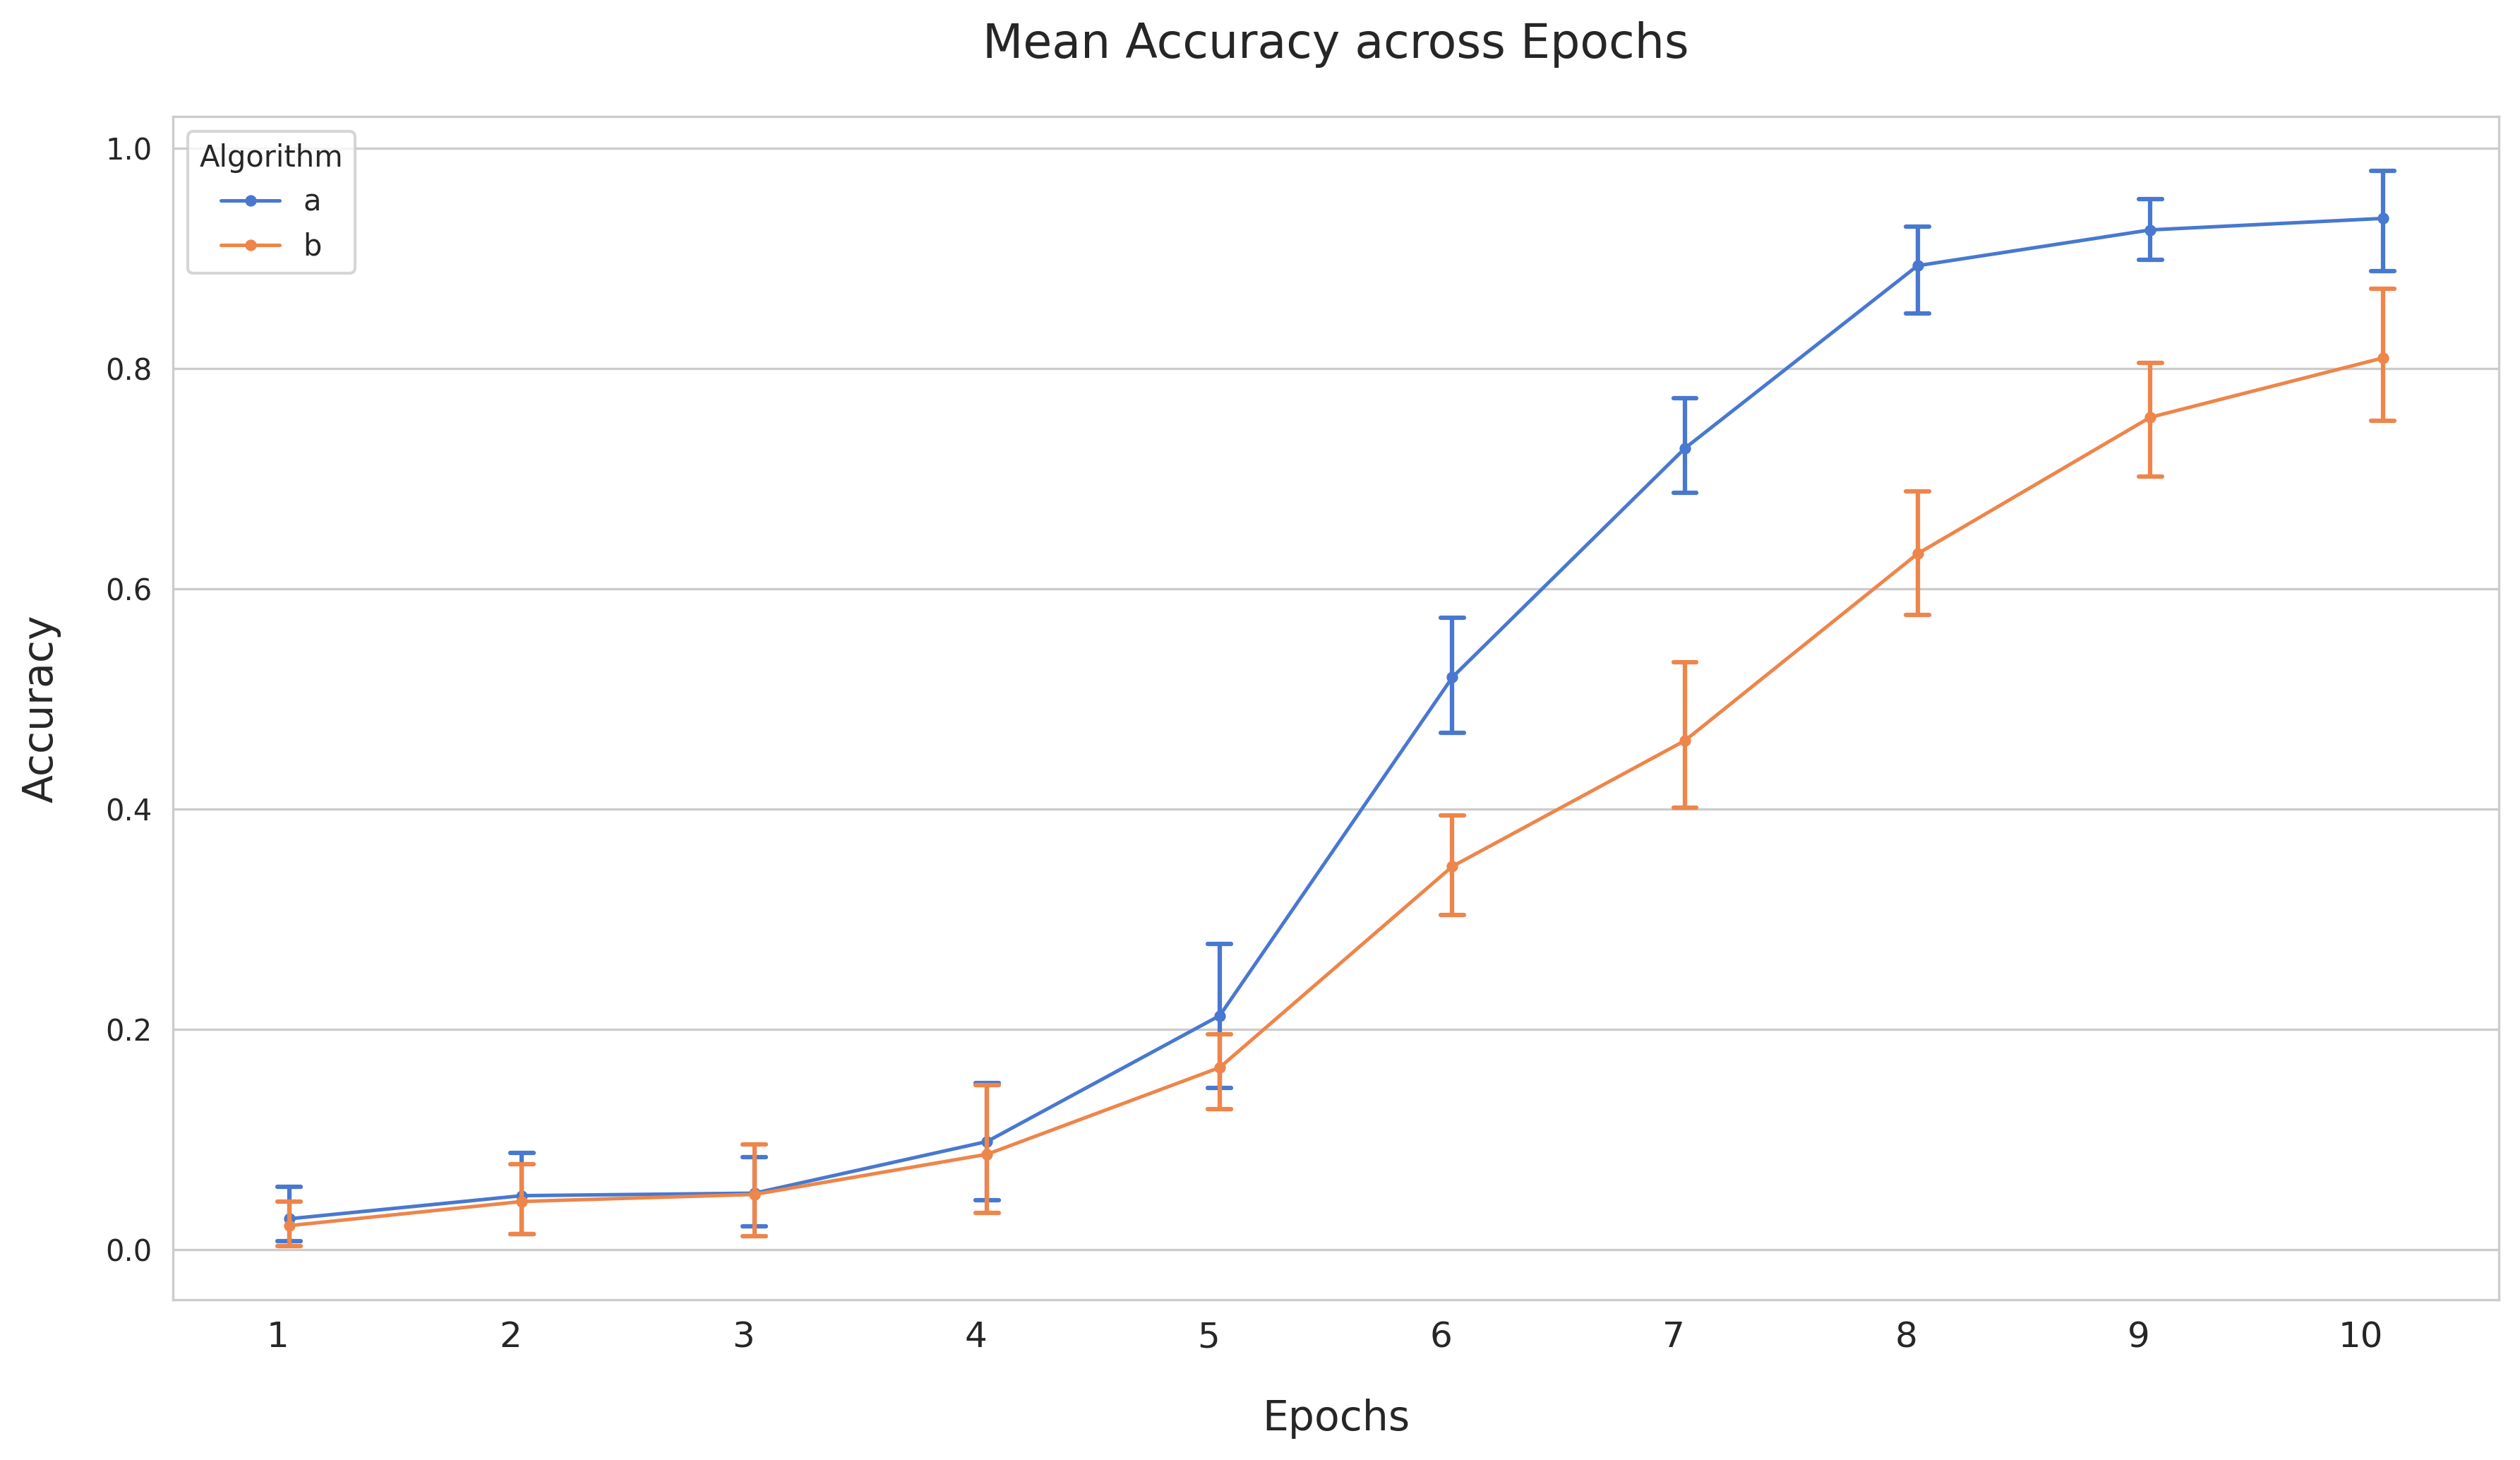
\includegraphics[width=0.95\textwidth]{figures/algo_accuracy_by_epoch_error_bar_plot.png}
  
  \textbf{Figure 13:} Mean Accuracy across Epochs by Algorithm with 95\% confidence intervals.
\end{center}

\textbf{Barcode Chart}
\begin{center}
  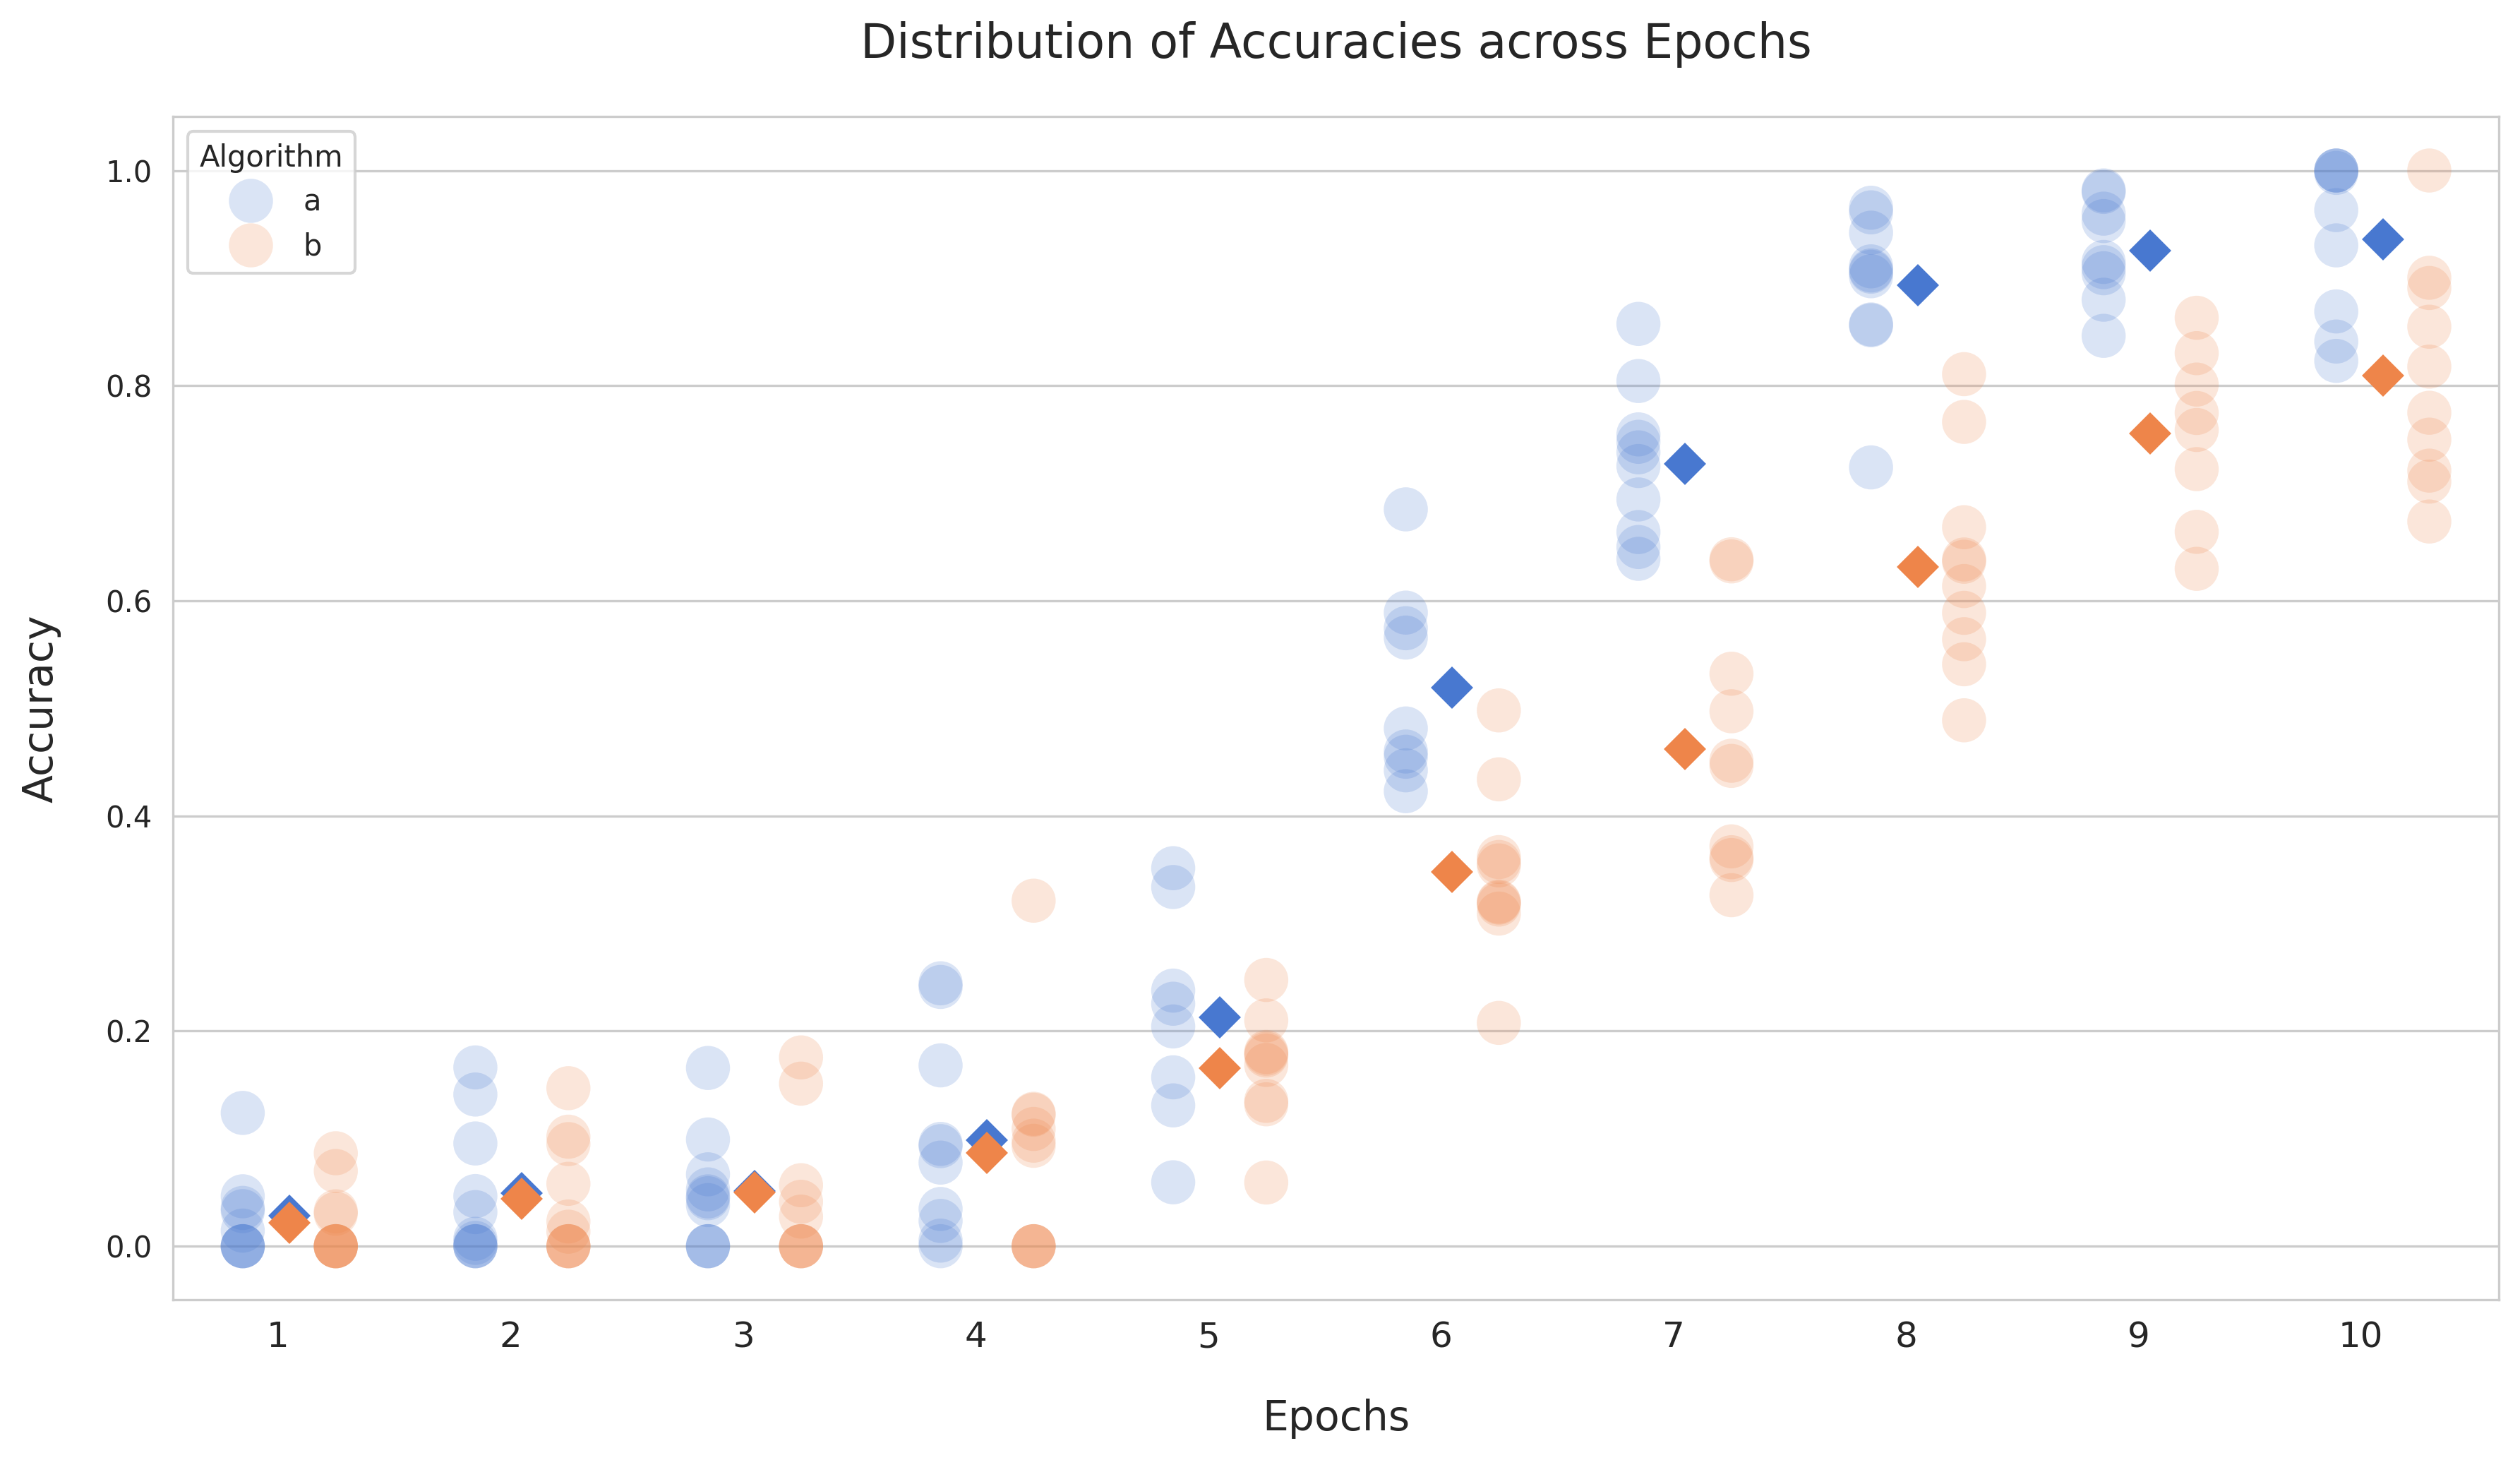
\includegraphics[width=0.95\textwidth]{figures/algo_accuracy_by_epoch_strip_plot.png}
  
  \textbf{Figure 14:} Average Distribution of Accuracy across Epochs by Algorithm.
\end{center}

\textbf{Histogram}
\begin{center}
  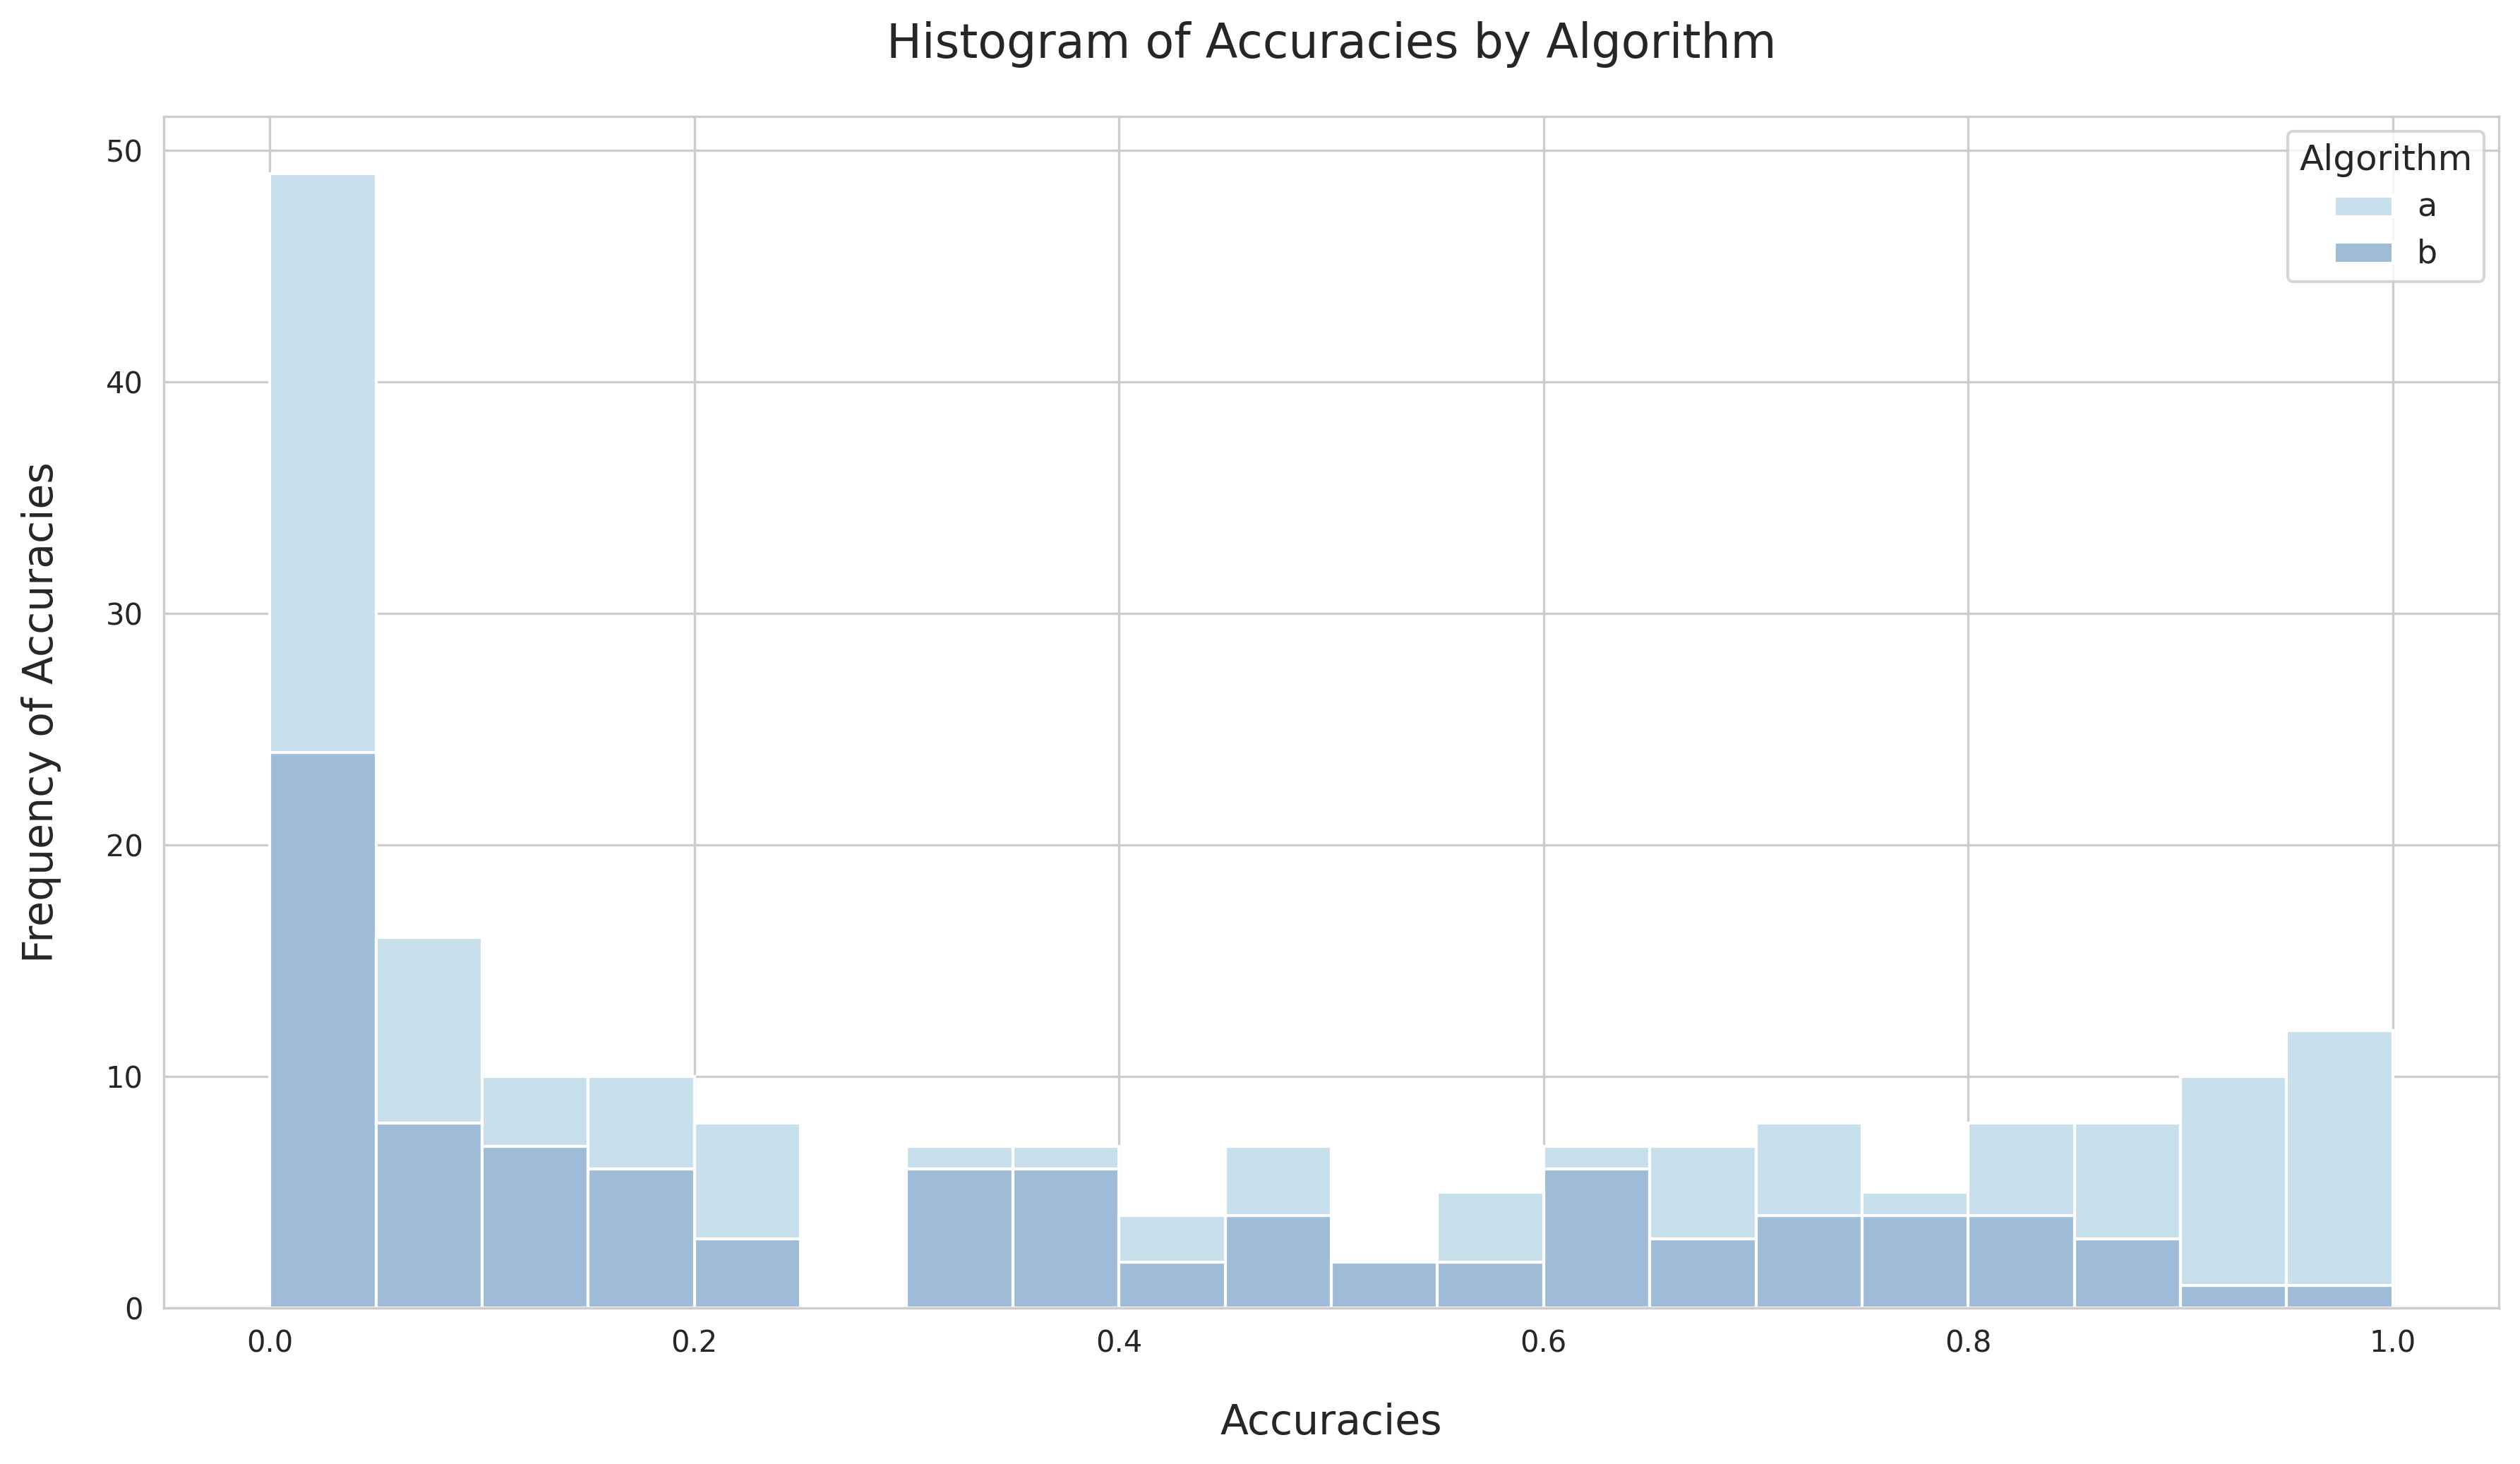
\includegraphics[width=0.95\textwidth]{figures/algo_accuracy_by_epoch_histogram_plot.png}
  
  \textbf{Figure 15:} Histogram of Accuracies by Algorithm.
\end{center}
\newpage

\subsection{Part C: Evaluate and Justify Visualization}
For the dataset:
\begin{itemize}
    \item Discuss the advantages and disadvantages of each visualization type.
    \item Decide which visualization is best for the research question.
    \item Support your answer with evidence from the plots and reasoning based on dataset size, shape, or structure.
\end{itemize}
-----\\
\textbf{Advantages and Disadvantages}\\
The error bar plot shows sample means plotted across each epoch, one plot for each algorithm. This gives us a clear comparison of the average accuracy between the two algorithms over the training cycle, and in some of the later epochs, gives an informative suggestion of how much more accurate algorithm A becomes over algorithm B. The error bar plot is quite uninformative in the whole first half of the training however. The comparable size of the error bars between the two algorithms means that we are not told much at all in terms of their difference from epochs 1-5. Nonetheless, we do get a decent representation of each algorithm's reliability and variation in performance, as the errors bar signal how volatile the performance can be across separate training runs.\\

The strip plot does well to show us the variation in performance for the specific training runs observed in the dataset, providing very similar information to the error bar plot. Like the album sales dataset, we are not concerned with too many observations at each epoch, so the mass distribution is quite readable from the plot, and we can easily read the difference in average performance across epochs. One key benefit of this visualization though is the fact that we have knowledge of extreme outliers in the training runs for each epoch, which for a sparse dataset, allow us to speak on the average performance across epoch for each algorithm with an increased level of nuance i.e. algorithm A at epoch x shows a higher/lower accuracy than B, but possesses extreme outliers at y\% accuracy, so we may require additional data to make a more sound comparison of each algorithm at this stage of the training.\\

The histogram plot was quite challenging to visualize for this dataset, as binning by algorithm and plotting accuracy frequency by accuracy bins loses any context of how performance develops over the training cycle, which leaves us with a weak comparison of the performance of the algorithms by themselves. This plot is overall quite weak for this context, but we can extract from the distribution of mass for each algorithm ideas about where inflection points and extreme values in the accuracy development over the epochs may have occurred.\\ 

For some arbitrary algorithm plotted in this manner, let's say its data showed a generally linear increase in accuracy over 10 epochs. Then, we can expect its histogram visualization to show a very uniform distribution of mass. Now, consider there was an inflection in its accuracy; likely in the earlier stages of training before a learned pattern has emerged for the model. We may see accuracy bin(s) where there is no mass in the histogram, as they were skipped over in the training cycle. Additionally, if for some trials there were some number of extreme outliers, we would see additional mass distributed to the appropriate bins roughly corresponding to other epochs. However, the fact remains that we are left without direct context of performance across epochs, so even the claims we could try to support from this visualization would be weak.\\

\textbf{Which visualization is best for the research question}\\

Which algorithm performs more accurately on average across epochs, and how does the use of a visualization help you assess reliability and variation of each algorithm? The strip plot is best for answering this research question.\\

\textbf{Evidence-based Support for this answer}\\
The error bar plot is quite a strong visualization for this data with respect to the research question: we can assess the reliability and performance variation of each algorithm from the samples means and the somewhat tight errors bars at every stage of the training. We can speak to qualities such as how there is strong support that algorithm A very reliably achieves an accuracy of around 0.9 and levels out starting at around its seventh epoch, really converging after the eighth. We can also make claims about how the data confidently suggests that algorithm A performs more accurately in the latter half of training, and that the error bars at the last epoch suggest that there at least some possibility that the true means of each may be converging or that algorithm B could surpass A given a longer training, and so we have insights with which to motivate further analysis. It's also worth mentioning that the error bars are a very direct signal of reliability of the algorithms and are powerful in letting us make claims about the comparative accuracies over the training, which is very relevant to the research question.\\

An issue that remains with the error bar plot however is the small scale of our observations for each epoch. We saw with the album sales dataset that for a small number of examples the variance in those observations can have a great amount of influence over how large the error bars have to be to remain 95\% confident, and so our understanding of average case behavior of each algorithm at each epoch can be potentially misguided. It is not so much of an issue here as the observations do not contain too many outliers, but there are enough to suggest that there is necessary context missing that would help us answer our research question more effectively.\\

This is context we are provided by the strip plots. For example, in epoch 4 for algorithm B (orange) we see that the observations are separated into three different groupings, and the accuracy of algorithm A is just above that of B. The highest outlier at this epoch for algorithm B is reflected in a relatively wide error bar, but now equipped with this additional context, we can make a more accurate claim about how the average case accuracy compares at this epoch. With more examples, we may see a temporary higher average accuracy for algorithm B before the inflection of A hits in epoch 6, or we may confirm the lower mass densities generally seen for this epoch. Getting to the directly the mass distribution in this scenario provides so much leverage in understanding the reliability of each algorithm as well, as color density directly relates to a notion of how often the algorithm yields nearly the same accuracy at each epoch. For this reason, it is very similar to the abilities of the error bar plot, but with a higher degree of granularity befitting a sparse dataset. \\

The histogram plot as mentioned earlier is a very clear loser for this data context. There is nothing to directly identify from this plot; even the strong claims we can make do not come from metrics directly identified by the visualization, but are only suggested by how the mass is distributed for each accuracy bin. For example, we could identify the lack of any mass in the bin 0.25-0.3, for which we can see a clear inflection point if we reference one of the other visualizations, occurring between epoch 5 and 6. So we can at least identify potentially a mutual inflection point in the training performance for both algorithms, but we cannot speak to exactly when it occurs without the context of one of the other visualizations. We can also suggest that each algorithm's performance increases slowly to begin with due to the increase mass for each concentrated in the lowest bin, but it remains to be seen that this plot provides any useful information regarding how the accuracy of each algorithm compares over the course of the training.
\newpage
